\documentclass[12pt]{book}

\usepackage{natbib} % Tidies up citation numbers.
\usepackage[utf8]{inputenc}
\usepackage{graphicx}
\usepackage{pythonhighlight}
\usepackage{listingsutf8}
\usepackage{float}

%\def\UrlBreaks{\do\/\do-}
\usepackage[T1]{fontenc}
\usepackage{url}
\usepackage{breakurl}

\usepackage{pdfpages}

\lstset{
  extendedchars=true,
  language=java,
  basicstyle=\tiny\ttfamily,
  showspaces=false,
  showstringspaces=false,
    literate=
     {É}{{\'E}}{1}%
      {Á}{{\'A}}{1}%
      {Ã}{{\~A}}{1}%
      {Â}{{\^A}}{1}%
      {À}{{\`A}}{1}%
      {Ç}{{\,C}}{1}%
      {Ó}{{\'O}}{1}%
      {Í}{{\'I}}{1}%
      {Õ}{{\~O}}{1}%
      {Ú}{{\'U}}{1}%
      {ú}{{\'u}}{1}%
      {é}{{\'e}}{1}%
      {á}{{\'a}}{1}%
      {ã}{{\~a}}{1}%
      {à}{{\`a}}{1}%
      {â}{{\^a}}{1}%
      {ç}{{\,c}}{1}%
      {ó}{{\'o}}{1}%
      {í}{{\'i}}{1}%
      {õ}{{\~o}}{1}%
}

\definecolor{gray}{rgb}{0.4,0.4,0.4}
\definecolor{darkblue}{rgb}{0.0,0.0,0.6}
\definecolor{cyan}{rgb}{0.0,0.6,0.6}

\lstdefinelanguage{XML}
{
 numbers=left,
 numberstyle=\tiny,
 stepnumber=1,
 numbersep=8pt,
 morestring=[b]",
 morestring=[s]{>}{<},
 morecomment=[s]{<?}{?>},
 stringstyle=\color{black},
 identifierstyle=\color{darkblue},
 keywordstyle=\color{cyan},
 morekeywords={xmlns,version,type}% list your attributes here
}

\colorlet{punct}{red!60!black}
\definecolor{background}{HTML}{EEEEEE}
\definecolor{delim}{RGB}{20,105,176}
\colorlet{numb}{magenta!60!black}

\lstdefinelanguage{json}{
    basicstyle=\tiny\ttfamily,
    numbers=left,
    numberstyle=\tiny,
    stepnumber=1,
    numbersep=8pt,
    showstringspaces=false,
    breaklines=true,
    frame=lines,
    backgroundcolor=\color{background},
    literate=
     *{É}{{\'E}}{1}%
      {Á}{{\'A}}{1}%
      {Ã}{{\~A}}{1}%
      {Â}{{\^A}}{1}%
      {À}{{\`A}}{1}%
      {Ç}{{\,C}}{1}%
      {Ó}{{\'O}}{1}%
      {Í}{{\'I}}{1}%
      {Õ}{{\~O}}{1}%
      {Ú}{{\'U}}{1}%
      {ú}{{\'u}}{1}%
      {é}{{\'e}}{1}%
      {á}{{\'a}}{1}%
      {ã}{{\~a}}{1}%
      {à}{{\`a}}{1}%
      {â}{{\^a}}{1}%
      {ç}{{\,c}}{1}%
      {ó}{{\'o}}{1}%
      {í}{{\'i}}{1}%
      {õ}{{\~o}}{1}%
     {0}{{{\color{numb}0}}}{1}
      {1}{{{\color{numb}1}}}{1}
      {2}{{{\color{numb}2}}}{1}
      {3}{{{\color{numb}3}}}{1}
      {4}{{{\color{numb}4}}}{1}
      {5}{{{\color{numb}5}}}{1}
      {6}{{{\color{numb}6}}}{1}
      {7}{{{\color{numb}7}}}{1}
      {8}{{{\color{numb}8}}}{1}
      {9}{{{\color{numb}9}}}{1}
      {:}{{{\color{punct}{:}}}}{1}
      {,}{{{\color{punct}{,}}}}{1}
      {\{}{{{\color{delim}{\{}}}}{1}
      {\}}{{{\color{delim}{\}}}}}{1}
      {[}{{{\color{delim}{[}}}}{1}
      {]}{{{\color{delim}{]}}}}{1},
}

\lstdefinelanguage{SPARQL}{
    basicstyle=\tiny\ttfamily,
    numbers=left,
    numberstyle=\tiny,
    stepnumber=1,
    numbersep=8pt,
    showstringspaces=false,
    breaklines=true,
    frame=lines,
    backgroundcolor=\color{background},
    literate=
     {É}{{\'E}}{1}%
      {Á}{{\'A}}{1}%
      {Ã}{{\~A}}{1}%
      {Â}{{\^A}}{1}%
      {À}{{\`A}}{1}%
      {Ç}{{\,C}}{1}%
      {Ó}{{\'O}}{1}%
      {Í}{{\'I}}{1}%
      {Õ}{{\~O}}{1}%
      {Ú}{{\'U}}{1}%
      {ú}{{\'u}}{1}%
      {é}{{\'e}}{1}%
      {á}{{\'a}}{1}%
      {ã}{{\~a}}{1}%
      {à}{{\`a}}{1}%
      {â}{{\^a}}{1}%
      {ç}{{\,c}}{1}%
      {ó}{{\'o}}{1}%
      {í}{{\'i}}{1}%
      {õ}{{\~o}}{1},%
  morekeywords={
    SELECT,CONSTRUCT,DESCRIBE,ASK,WHERE,FROM,NAMED,PREFIX,BASE,OPTIONAL,
    FILTER,GRAPH,LIMIT,OFFSET,SERVICE,UNION,EXISTS,NOT,BINDINGS,MINUS,a
  }
}

\lstdefinelanguage{overpassQL}{
    basicstyle=\tiny\ttfamily,
    numbers=left,
    numberstyle=\tiny,
    stepnumber=1,
    numbersep=8pt,
    showstringspaces=false,
    breaklines=true,
    frame=lines,
    backgroundcolor=\color{background}
}

\lstset{language=R,
    literate=
    {<-}{{$\gets$}}1%
     {É}{{\'E}}{1}%
      {Á}{{\'A}}{1}%
      {Ã}{{\~A}}{1}%
      {Â}{{\^A}}{1}%
      {À}{{\`A}}{1}%
      {Ç}{{\,C}}{1}%
      {Ó}{{\'O}}{1}%
      {Í}{{\'I}}{1}%
      {Õ}{{\~O}}{1}%
      {Ú}{{\'U}}{1}%
      {ú}{{\'u}}{1}%
      {é}{{\'e}}{1}%
      {á}{{\'a}}{1}%
      {ã}{{\~a}}{1}%
      {à}{{\`a}}{1}%
      {â}{{\^a}}{1}%
      {ç}{{\,c}}{1}%
      {ó}{{\'o}}{1}%
      {í}{{\'i}}{1}%
      {õ}{{\~o}}{1},%
    basicstyle=\tiny\ttfamily,
    stringstyle=\color{red},
    otherkeywords={0,1,2,3,4,5,6,7,8,9},
    morekeywords={TRUE,FALSE},
    deletekeywords={data,frame,length,as,character},
    keywordstyle=\color{blue},
    commentstyle=\color{red},
}

\usepackage[brazil]{babel}  
\usepackage{xcolor}
%xcolor v2.12 (2016/05/11)384  Colors by Name4.1  Base colors (always available)black blue brown cyan darkgray gray green lightgray lime magenta olive orange pink purple red teal violet white yellow

\usepackage[nopostdot]{glossaries}
\setglossarystyle{altlist}
\PassOptionsToPackage{hyphens}{url}
\usepackage [colorlinks = true,
            linkcolor = blue,
            urlcolor  = blue,
            citecolor = blue,
            anchorcolor = blue]{hyperref} 

% gerador de lero-lero
\usepackage{lipsum}

\usepackage{pdfpages}

\newenvironment{itquote}
{\begin{quote}\itshape}
{\end{quote}}

\usepackage[commentmarkup=todo]{changes}

\usepackage{datetime2}

\usepackage{booktabs}

\usepackage{caption}
\input{packages-estudantes}

% define cores personalizadas para o texto de cada autor
\usepackage
%[final]
{changes}
%\usepackage{changes}
%\url{https://ctan.org/pkg/changes}

\definechangesauthor[name={Jorge Henrique Cabral Fernandes}, color=orange]{jhcf} % git-user: jhcf

\definechangesauthor[name={Alexsander Correa de Oliveira}, color=black]{KvotheKS} % git-user: KvotheKS OK

\definechangesauthor[name={Allann Gois Hoffmann}, color=orange]{AllannH} % git-user: AllannH OK

\definechangesauthor[name={André Larrosa Chimpliganond}, color=orange]{andrelarrosacrypt} % git-user: andrelarrosacrypt OK

\definechangesauthor[name={André Cássio Barros de Souza}, color=green]{andreloff} % git-user: andreloff OK

\definechangesauthor[name={Bruno Sanguinetti Regadas de Barros}, color=blue]{Jaxiii} % git-user: Jaxiii OK

\definechangesauthor[name={Enzo Nunes Leal Sampaio}, color=orange]{enzodevs2000} % git-user: enzodevs2000 OK

\definechangesauthor[name={Felipe Gomes Paradas}, color=pink]{fparadas} % git-user: fparadas OK

\definechangesauthor[name={Lucas de Almeida Bandeira Macedo}, color=teal]{ABMHub} % git-user: ABMHub OK

\definechangesauthor[name={Fernanda Macedo de Sousa}, color=magenta]{fernandams} % git-user: fernandams Ok

\definechangesauthor[name={Gabriel dos Santos Martins}, color=green]{gsmartins96} %  git-user: gsmartins96 OK

\definechangesauthor[name={Gabriel Faustino Lima da Rocha}, color=gray]{Faustino27} %  git-user: Faustino27 OK

\definechangesauthor[name={Gabriel Martins de Almeida}, color=purple]{GMalme} %  git-user: GMalme OK

\definechangesauthor[name={Gabriel Rocha Fontenele}, color=pink]{ngsylar} % git-user: ngsylar OK

\definechangesauthor[name={Ítalo Eduardo Dias Frota}, color=pink]{titofrota} % git-user: titofrota OK

\definechangesauthor[name={João Antonio Desidério de Moraes}, color=teal]{joaoadm94} % git-user: joaoadm94 OK

\definechangesauthor[name={Ualiton Ventura da Silva}, color=orange]{uventura} % git-user: uventura OK

\definechangesauthor[name={Pedro de Torres Maschio}, color=orange]{pedro-maschio} % git-user: pedro-maschio OK

\definechangesauthor[name={Tong Zhou}, color=orange]{Tong00020} % git-user: Tong00020 Ok

\definechangesauthor[name={Gustavo Rodrigues dos Santos}, color=pink]{gutorsantos} % git-user: gutorsantos OK

\definechangesauthor[name={Gustavo Tomás de Paula}, color=green]{gustavo-tomas} % git-user: gustavo-tomas OK

\definechangesauthor[name={Gustavo Macedo de Carvalho}, color=purple]{GustavoMacCar} % git-user: GustavoMacCar OK

\definechangesauthor[name={Arthur da Silveira Couto}, color=purple]{CrimsonCrown} % git-user: CrimsonCrown OK?

\definechangesauthor[name={Vitor de Oliveira Araujo Araruna}, color=orange]{vitorararuna} % git-user: vitorararuna OK

\definechangesauthor[name={Rafael dos Santos Silva}, color=red]{rafaelsilva21} % git-user: rafaelsilva21 OK

\definechangesauthor[name={Marcus Vinicius Oliveira de Abrantes}, color=red]{MarcusABR} % git-user: MarcusABR OK

\definechangesauthor[name={Mateus de Paula Rodrigues}, color=cyan]{MoustacheGolem} % git-user: MoustacheGolem OK

\definechangesauthor[name={Leonardo Alves Riether}, color=blue]{LeoRiether} % git-user: LeoRiether OK

\definechangesauthor[name={Tatiana Franco Pereira}, color=cyan]{Tatianafp} % git-user: Tatianafp OK

\definechangesauthor[name={Vinícius Caixeta de Souza}, color=orange]{vinis-caixe} % git-user: vinis-caixe OK

\definechangesauthor[name={Conrado Nunes Barbosa Neto}, color=blue]{Conras21} % git-user: Conras21 OK

\definechangesauthor[name={Stefano Luppi Sposito}, color=pink]{KawaiiStheno} % git-user: KawaiiStheno OK

\definechangesauthor[name={João Pedro Felix de Almeida}, color=teal]{DYosplay} % git-user: DYosplay OK

\definechangesauthor[name={João Víctor Siqueira de Araujo}, color=red]{StrawHat972} % git-user: StrawHat972 OK

\definechangesauthor[name={Raylan da Silva Sales}, color=pink]{Rayxan} % git-user: Rayxan OK

\definechangesauthor[name={Guilherme Oliveira Loiola}, color=blue]{guioliunb} % git-user: guioliunb OK

\definechangesauthor[name={Paulo Alvim Alvarenga}, color=purple]{alvimpaulo} % git-user: alvimpaulo OK

\definechangesauthor[name={Léo Akira Abe Barros}, color=red]{leoakir} % git-user: leoakir OK

\definechangesauthor[name={Enzo Yoshio Niho}, color=purple]{enzoyoshio} % git-user: enzoyoshio OK

\definechangesauthor[name={Daniel Rodrigues Cardoso}, color=blue]{DanielrCardoso} % git-user: DanielrCardoso OK

\definechangesauthor[name={Fernando Ferreira Cordeiro}, color=blue]{FernandoCordeiro} % git-user: FernandoCordeiro OK

\definechangesauthor[name={Jônatas Gomes Barbosa da Silva}, color=cyan]{jonatas1n} % git-user: jonatas1n OK

\definechangesauthor[name={Lucas Gabriel de Oliveira Gurgel Fernandes}, color=black]{lggurgel} % git-user: lggurgel OK

\definechangesauthor[name={Bruno Esteves Dalla Costa Filho}, color=red]{brunoedcf} % git-user: brunoedcf OK

\definechangesauthor[name={Paulo Mauricio Costa Lopes}, color=red]{RequiemDosVivos} % git-user: RequiemDosVivos OK

\definechangesauthor[name ={Caio Bernardon Nascif Kaawi Massucato}, color=blue]{CaioMassucato} % git-user: CaioMassucato OK 

\makenoidxglossaries
\loadglsentries{1-Introducao/tarefas/1.1-Glossario/estudantes/main}
\setcounter{tocdepth}{5}
\setcounter{secnumdepth}{5}
\captionsetup[table]{name=Quadro}
\renewcommand{\lstlistingname}{Listagem de Código}

\newcommand{\dataset}{\textit{dataset}}
\newcommand{\query}{\textit{query}}
\newcommand{\githubusername}{\textless githubusername\textgreater}

\begin{document}

\chapter{Análise Bibliográfica sobre O auxílio da indústria dos jogos na evolução do Hardware, por Gabriel Martins de Almeida}

\section{Planejamento do estudo}

Este é um projeto com o propósito de treinar o uso de técnicas de análises bibliométricas para fins de aprendizado. Em resumo, vivemos em um mundo altamente integrado com a tecnologia e embora muitos profissionais, por exemplo, um design gráfico necessita de um processador potente para ter uma boa eficiência no seu trabalho, um usuário comum não necessita do mesmo para o seu ambiente profissional, mas os jogos acabam por levar está necessidade para os clientes usuais. Logo, o lazer relacionado aos jogos aumenta a busca por hardware , então o objetivo é responder as seguintes perguntas.

\begin{itemize}
    \item Quais são os principais usos para o hardware comprado por consumidores comuns?
    \item A evolução do hardware e o aumento dos requisitos de sistemas para jogos estão relacionados?
    \item Com a popularização dos jogos o preço do hardware subiu ou desceu? Quais acontecimentos podem está ligado a esta possível variação?
\end{itemize}

\subsection{Limitações} As limitações estão relacionadas ao tempo, pois é uma atividade introdutória então não foi possível ler os artigos resultantes das buscas e a falta de experiência com a ferramenta pode levar a alguns resultados inesperados.

\section{Coleta de dados} 
Os dados foram coletados na base de dados Web of Science no dia 9 de fevereiro de 2022, acessado por meio do Portal de Periódicos da CAPES

\subsection{Query de Busca}
\begin{verbatim}
A query utilizada para a busca foi:
(game* or  specification or requirements ) 
and 
(advances or computer) 
and 
(hardware or purchase)
\end{verbatim}

\subsection{Explicação para os termos de busca usados}

O primeiro termo utilizado busca informações sobre requisitos e especificações para determinado jogo sendo utilizado o termo game* para buscar dados sobre um jogo e também podendo retornar uma busca para as especificações e requisitos relacionados aos jogadores. O segundo termo busca relacionar o termo a avanços tecnológicos na computação que também está relacionado ao tema da pesquisa, o terceiro tem o proposito de complementar os anteriores tentando buscar informações sobre compras de componentes.

\subsection{Registros recuperados}

A busca retornou 6858 resultados, sendo utilizado uma exportação personalizada passando também como parâmetro as referências citadas, contagem de referências citadas, total de usos e artigos interessantes. Logo, foi feita uma exportação de 5 arquivos de texto sem formatação com um tamanho de 1000 registros e após foi realizada uma concatenação em apenas um arquivo para ser possível passar os 6858 resultados da pesquisa para o biblioshiny.

\section{Análise dos dados}

\subsection{Filtragem de registros}
Após uma filtragem que deu enfoque para os artigos científicos retirando, por exemplo, notas, artigos com acesso antecipado, avaliações de software, etc. foi possível reduzir o número de resultados para 2233.

\subsection{Análise descritiva do dataset}

A descrição das informações principais são:

\begin{description}
    \item [\textit{Timespan}] Os artigos obtidos após a filtragem foram publicados entre o período de 1971 até 2022
    \item [\textit{Sources (Journals, Books, etc)}] Os artigos possuem ao todo 1119 fontes diferentes.
    \item [\textit{Average years from publication}] A média de tempo de publicação dos artigos é de 10.6 anos
    \item [\textit{Average citations per documents}] A média de citações por documentos é 17.33.
    \item [\textit{Average citations per year per doc}] Após o ano de sua publicação, das um dos dos artigos foi citado em média 1.689 vezes por ano.
    \item [\textit{References}] Ao todo, foram feitas 68302 referências por entre os artigos coletados
    \item [\textit{Keywords Plus (ID)}] 0 palavras chaves do tipo ID (Keyword Plus)
    \item [\textit{Author's Keywords (DE)}]  0 palavras chaves escolhidas pelos autores dos artigos

    \item [\textit{Authors}]  são 8105 autores
    \item [\textit{Author Appearances}] 8722
    \item [\textit{Authors of single-authored documents}] Dos 8105 autores, 263 escreveram artigos individualmente
    \item [\textit{Authors of multi-authored documents}] Dos 8105 autores, 263 são autores de artigos escritos em colaboração com outros.
    \item [\textit{Single-authored documents}] São 268 documentos escritos individualmente
    \item [\textit{Documents per Author}] A média de documentos por autor é de 0.276
    \item [\textit{Authors per Document}] A média de autores por documento é de 3.63.
    \item [\textit{Co-Authors per Documents}] As 5749 aparições de autores se distribuem em 3.91 por documento
    \item [\textit{Collaboration Index}] O indíce de colaboração (total de autores em artigos escritos em co-autoria / total de artigos escritos em co-autoria) é de 3.99.
\end{description}


\subsection{Evolução da Produção Científica}

\begin{figure}[ht]
    \centering
    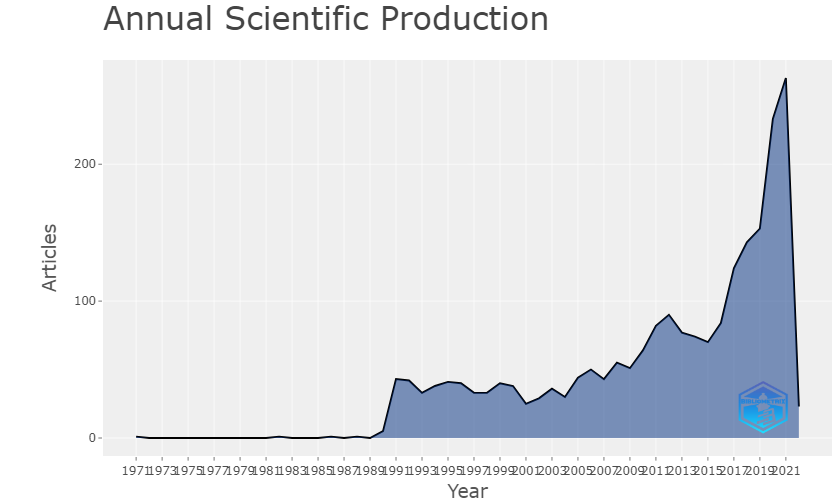
\includegraphics[width=12cm]{experiments/GMalme/AnaliseBibliometrica/ImpactoDeJogosNaTecnologia/Figs/Annual Scientific Production.png}
    \caption{Produção cientifica anual}
    \label{fig:AIJ_produçãoAnual}
\end{figure}

\subsection{Evolução da Produção Científica}

\begin{figure}[ht]
    \centering
    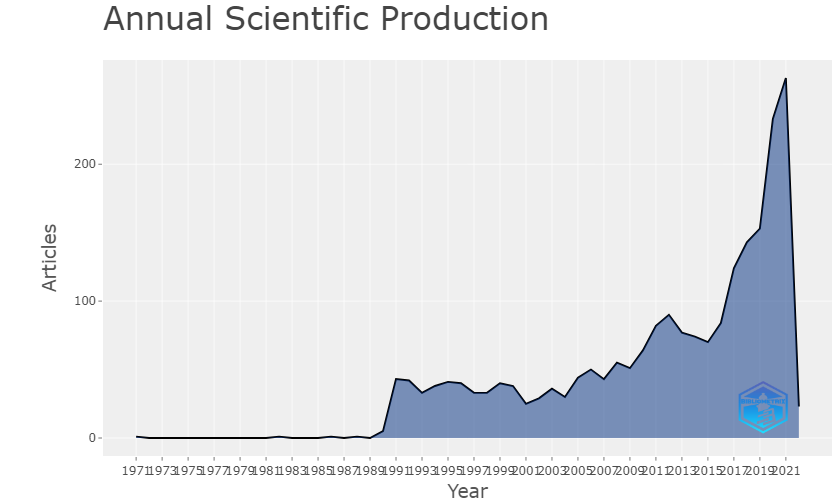
\includegraphics[width=12cm]{experiments/GMalme/AnaliseBibliometrica/ImpactoDeJogosNaTecnologia/Figs/Annual Scientific Production.png}
    \caption{Produção cientifica anual}
    \label{fig:AIJ_produçãoAnual}
\end{figure}

\subsection{Evolução da Produção Científica}

\begin{figure}[ht]
    \centering
    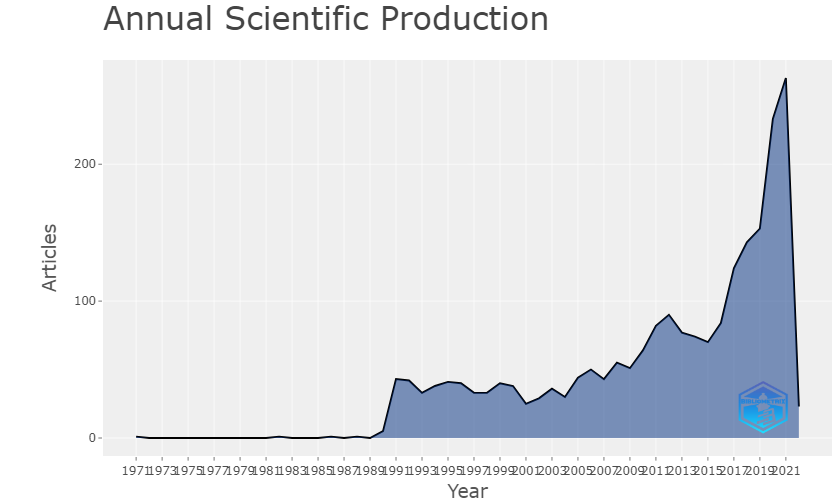
\includegraphics[width=12cm]{experiments/GMalme/AnaliseBibliometrica/ImpactoDeJogosNaTecnologia/Figs/Annual Scientific Production.png}
    \caption{Produção cientifica anual}
    \label{fig:AIJ_produçãoAnual}
\end{figure}




\bibliographystyle{plainnat}
\bibliography{RESIC}

\end{document}.
